\section{Adding New Services: Step-By-Step}
\begin{enumerate}
\item Make copies of the service template source and header files:
\begin{docspec}
    uxas/code/src/Services/00\_ServiceTemplate.cpp
\end{docspec}
\begin{docspec}
    uxas/code/src/Services/00\_ServiceTemplate.h
\end{docspec}
\item Change the name of the copied files to reflect the name of the new service.
\item In the new files, search for the string \textit{c00\_ServiceTemplate} and Replace it with the new service name.
\item Change the unique include guard entries in the header file, i.e. \textit{UXAS\_00\_SERVICE\_TEMPLATE\_H}, to match the new service name.
\item Edit the file:
\begin{docspec}
    uxas/code/src/Services/00\_ServiceList.h
\end{docspec}
to add entries for the new service:
\begin{enumerate}
  \item include the header file for the new service in the section labeled \textit{SERVICE HEADER FILES SECTION}, e.g.:
\begin{docspec}
\#include "CmasiAreaSearchTaskService.h"
\end{docspec}
  
  \item add a service registration string in the section labeled \textit{SERVICE REGISTRATION SECTION} e.g.:
\begin{docspec}
{auto svc = uxas::stduxas::make\_unique<afrl::cmasi::AreaSearchTask>();}
\end{docspec}
  \item if the new service is a task, include the header file of the corresponding task message in the section labeled \textit{INCLUDE TASK MESSAGES SECTION}, e.g.:
\begin{docspec}
\#include "afrl/cmasi/AreaSearchTask.h"
\end{docspec} 
  \item if the new service is a task, add a subscription string in the section labeled \textit{SUBSCRIBE TO TASKS SECTION}, e.g.:
\begin{docspec}
addSubscriptionAddress(afrl::cmasi::AreaSearchTask::AREASEARCHTASK\_FULL\_LMCP\_TYPE\_NAME);
\end{docspec} 
  \end{enumerate}  
\end{enumerate}


\section{Configuring Services}
Service are configured using a global configuration file written in XML. The configuration file is selected either  by using the default configuration file name: \textbf{\textit{cfg.xml}} or passing in the path/filename when starting UxAS:
\begin{docspec}
	uxas\_main \textbf{-cfgPath} \textit{../PathToConfigurationFile/cfgFileName.xml}
\end{docspec} 
The elements contained in an UxAS configuration file are, \textbf{XML Declaration}, \textbf{UxAS Element}, \textbf{Service Elements}, and \textbf{Bridge Elements}, see Figure \ref{fig:configExample}. 
\begin{marginfigure}[-100pt]
	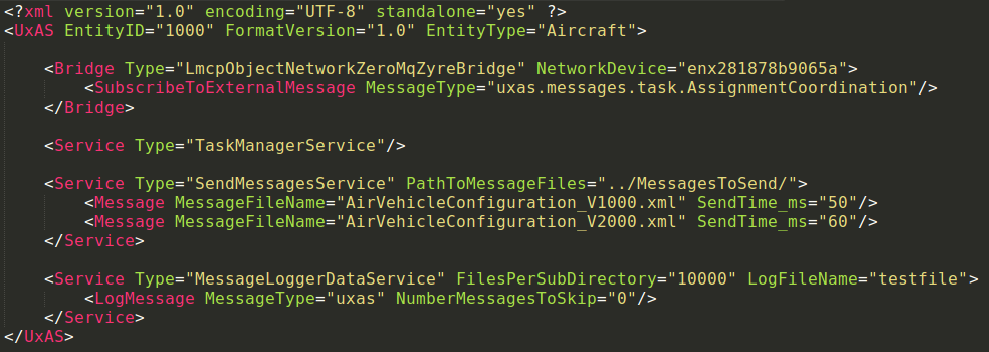
\includegraphics[width=1.3\linewidth]{\FiguresPath//ConfigExample}
	\caption{Sample configuration file}
	\label{fig:configExample}
\end{marginfigure}

Here is the \textbf{XML Declaration}:
\begin{docspec}<?xml version="1.0" encoding="UTF-8" standalone="yes" ?>\end{docspec}
The \textbf{UxAS Element}:
\begin{docspec}
	<UxAS EntityID="1000" FormatVersion="1.0" EntityType="Aircraft">
\end{docspec}
accepts the following attributes:
\begin{description}
	\item[\textit{EntityID}] Identification number of the entity represented by this instance of UxAS
	%\item[\textit{FormatVersion}] description ??????
	\item[\textit{EntityType}] used to differentiate between entities such as, \textit{Aircraft} and \textit{UGS}. Entries are defined by the services that use them.
	\item[\textit{ConsoleLoggerSeverityLevel}] if this attribute is present, all log messages at or below the severity level are displayed in the console. Valid entries are: \textit{DEBUG}, \textit{INFO}, \textit{WARN}, and \textit{ERROR}
	\item[\textit{MainFileLoggerSeverityLevel}] if this attribute is present, all log messages at or below the severity level are save in log files. Valid entries are: \textit{DEBUG}, \textit{INFO}, \textit{WARN}, and \textit{ERROR}
	%\item[\textit{StartDelay\_ms}] description
	\item[\textit{RunDuration\_s}] UxAS will run for \textit{RunDuration\_s} seconds before terminating.
	%\item[\textit{isLoggingThreadId}] description
\end{description}
Service Elements configure the services. There can be as many Service Elements as required. The attributes of the Service Elements are the options defined by each service. For example, the HelloWorld service can be configured with the following Service Element:
\begin{docspec}
	<Service Type="HelloWorld" StringToSend="Hello from \#1" SendPeriod\_ms="1000"/>
\end{docspec}
Bridge Elements configure bridges, which are services that create communication connections. For the Distributed Cooperation example, the zyre connection is configured with the following Bridge Element:
\begin{docspec}
    <Bridge Type="LmcpObjectNetworkZeroMqZyreBridge" NetworkDevice="enx281878b9065a">
	\quad<SubscribeToExternalMessage MessageType="uxas.messages.task.AssignmentCoordination"/>
	</Bridge>
\end{docspec}



\section{Core Services}\label{core-services}

The core services of UxAS work in concert to carry out the \emph{task assignment pipeline}
which automates the calculation of the proper vehicle-task orderings for efficient overall
mission completion. The design choice to seperate each of these services is motivated by
consideration of computational complexity as well as availability in the literature for
parts of the process (i.e. route planners and task assignment algorithms).

\begin{figure*}
	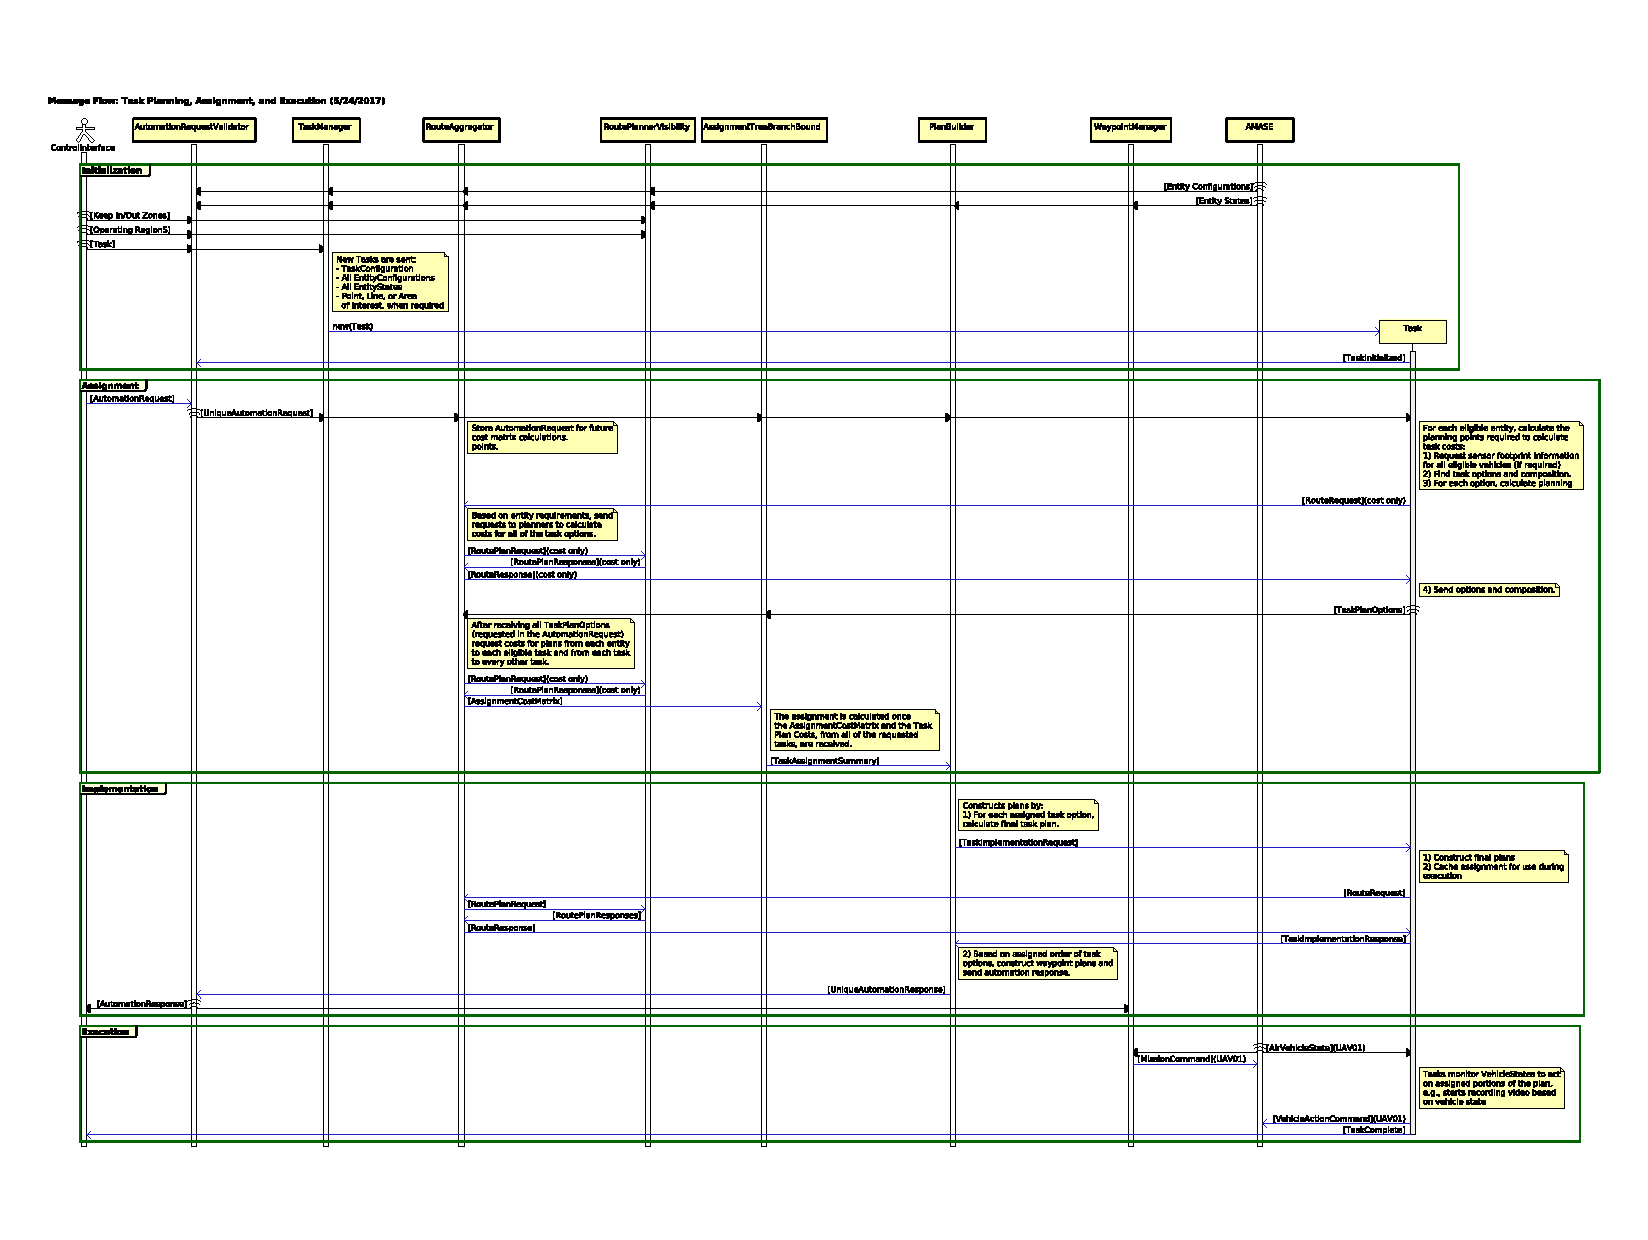
\includegraphics[width=1.0\linewidth]{\CCAFiguresPath//CCA_Components_MessageFLow}
	\caption{Message Flow for Task Assignment Pipeline}
	\label{fig:CoreServiceMessageFlow}
\end{figure*}

The message flow between the core services is captured in Figure~\ref{fig:CoreServiceMessageFlow}
and indicates the temporal relationship between the core services in carrying out a complete
automation request. Time proceeds from the top of the diagram to the bottom with
each horizontal arrow representing a single LMCP message of the specified type.

\begin{description}
\item
  \textbf{\textit{AutomationRequestValidatorService}} - This service will check an outside
  automation request for feasibility. If any task, vehicle, or operating region in the request
  has not yet been described to the system, this service will return an error indicating that
  the request cannot be fulfilled. If all necessary parts of the request are available to the
  system, then this service will attach a unique identifier to the request and start the
  sequence of steps necessary to fulfill that request. If any other outside requests are made
  while the system is in the process of fulfilling an existing request, this service will queue
  those additional requests, ensuring that the system only handles one request at a time. 
\item
  \textbf{\textit{TaskManagerService}} - This service dynamically creates new task services as
  their descriptions are sent into the system. When a new \textit{Task} is described, this service
  will send the proper configuration message for construction of a new service that adheres to
  the general task interface specification for that particular \textit{Task}. As part of the task
  service construction, this service will pass along all relevant details that a \textit{Task}
  needs for calculation of its behavior (i.e. current vehicle states, defined areas of interest, etc).
\item
  \textbf{\textit{Task}} - Tasks make up the atomic building blocks of automation requests. The
  composition of tasks and the assignment of particular vehicles to tasks comprises an automation
  response. When included as part of an automation request, a \textit{Task} reports a set of
  possible \emph{options} which represent the possible ways that the task can be completed. Each
  option is precisely a start and end location for applicable vehicles as well as the cost to
  complete the task using that option. The location and cost information for each option is used
  by the assignment service to select an option for each task that completes the overall mission
  efficiently. Once an option is selected by the assignment service, each \textit{Task} also
  reports the set of waypoints that a vehicle should use to complete the task.
\item
  \textbf{\textit{RoutePlannerVisibilityService}} - One of potentially many route planners, this
  service fulfills simple requests for routing in complex environments. For a given environment
  (described by sets of \textit{KeepIn} and \textit{KeepOut} polygons), a route planner will
  calculate the appropriate waypoints to guide a vehicle from a prescribed start location to a
  desired end location, ensuring that no waypoint is placed in an invalid area. This particular
  route planner uses a visibility graph as a basis to create distance-minimizing routes in two
  dimensions. Route planning services have a simple request-reply interface with each request
  corresponding to a single vehicle in a single environment.
\item
  \textbf{\textit{RouteAggregatorService}} - This service works with a set of route planners,
  requesting routes from the appropriate planner based on the situation. Additionally, this service
  provides the capability to make large-scale route planning requests involving multiple vehicles
  and multiple start/end locations. A primary use of this service is to calculate routes for all
  vehicles to travel between task locations. By orchestrating the cost-to-go calculations
  between tasks, this service acts as the bookkeeper for the complete cost map required by
  assignment algorithms.
\item
  \textbf{\textit{AssignmentTreeBranchBoundService}} - This service provides a resource allocation
  algorithm to determine an efficient use of the vehicle assets to fulfill tasks in the system. By
  design, the resource allocation is de-coupled from route planning and only uses the costs
  provided by the \textit{RouteAggregatorService}. The ultimate output of this service is an ordered
  list of tasks for each vehicle. This ordering must account for the process algebra relationship
  between tasks. This particular assignment service builds a tree of possible assignment orderings
  and prunes that tree based on the prescribed task relationships. The algorithm proceeds in two phases:
  1) greedy, depth-first search to find a feasible plan; 2) backtracking up the tree in a
  branch-and-bound manner to discover plans that are lower cost than the initial greedy plan. Once a
  predetermined amount of the tree has been searched (to ensure worst-case execution time), the
  assignment service will return the most efficient task ordering discovered.
\item
  \textbf{\textit{PlanBuilderService}} - With a task ordering determined by the assignment service,
  the \textit{PlanBuilderService} will organize the final set of waypoints that each vehicle should
  follow to complete the assignment. Working through the task ordering, this service requests the
  appropriate \textit{Tasks} in the assigned order to build a complete set of waypoints for each
  vehicle to carry out the mission. By stitching each part of the mission together in the proper
  order, this service provides the automation response that fulfills the original, outside
  automation request.
\end{description}

What follows are details for each of the core services and a rough description of the state machines
that each follows to complete its part of the overall task assignment process. See the auto-generated
LMCP documentation for precise details of each message.

%% paste in pandoc output of CoreServices.md `pandoc -o CoreServices.tex CoreServices.md`  %%
\subsection{AutomationRequestValidatorService}\label{automationrequestvalidatorservice}

This service provides a simple sanity check on external automation
requests. It also queues requests and tags them with unique identifiers,
feeding them into the system one at a time.

This service has two states: \textbf{idle} and \textbf{busy}. In both
states, when a non \emph{AutomationRequest} message is received, a local
memory store is updated to maintain a list of all available tasks,
vehicle configurations, vehicle states, zones, and operating regions.

Upon reception of an \emph{AutomationRequest} message, this service
ensures that such a request can be carried out by checking its local
memory store for existence of the requested vehicles, tasks, and
operating region. If the request includes vehicles, tasks, or an
operating region that has not previously been defined, this service will
publish an error message.

Upon determination that the \emph{AutomationRequest} includes only
vehicles, tasks, and an operating region that have previously been
defined, this service creates a \emph{UniqueAutomationRequest} with a
previously unused unique identifier. If in the \textbf{idle} state, this
service will immediately publish the \emph{UniqueAutomationRequest}
message and transition to the \textbf{busy} state. If already in the
\textbf{busy} state, the \emph{UniqueAutomationRequest} will be added to
the end of a queue.

When this service receives either an error message (indicating that the
\emph{UniqueAutomationRequest} cannot be fulfilled or a corresponding
\emph{UniqueAutomationResponse}), it will publish the same message. If
in the \textbf{idle} state, it will remain in the \textbf{idle} state.
If in the \textbf{busy} state, it will remove from the queue the request
that was just fulfilled and then send the next
\emph{UniqueAutomationRequest} in the queue. If the queue is empty, this
service transitions back to the \textbf{idle} state.

This service also includes a parameter that allows an optional
\emph{timeout} value to be set. When a \emph{UniqueAutomationRequest} is
published, a timer begins. If the \emph{timeout} has been reached before
a \emph{UniqueAutomationResponse} is received, an error is assumed to
have occured and this service removes the pending
\emph{UniqueAutomationRequest} from the queue and attempts to send the
next in the queue or transition to \textbf{idle} if the queue is empty.

\begin{longtable}[c]{@{}ll@{}}
\caption{Table of messages that the
\emph{AutomationRequestValidatorService} receives and
processes.}\tabularnewline
\toprule
\begin{minipage}[b]{0.29\columnwidth}\raggedright\strut
Message Subscription
\strut\end{minipage} &
\begin{minipage}[b]{0.65\columnwidth}\raggedright\strut
Description
\strut\end{minipage}\tabularnewline
\midrule
\endfirsthead
\toprule
\begin{minipage}[b]{0.29\columnwidth}\raggedright\strut
Message Subscription
\strut\end{minipage} &
\begin{minipage}[b]{0.65\columnwidth}\raggedright\strut
Description
\strut\end{minipage}\tabularnewline
\midrule
\endhead
\begin{minipage}[t]{0.29\columnwidth}\raggedright\strut
\emph{AutomationRequest}
\strut\end{minipage} &
\begin{minipage}[t]{0.65\columnwidth}\raggedright\strut
Primary message to request a set of Tasks to be completed by a set of
vehicles in a particular airspace configuration (described by an
\emph{OperatingRegion}).
\strut\end{minipage}\tabularnewline
\begin{minipage}[t]{0.29\columnwidth}\raggedright\strut
\emph{EntityConfiguration}
\strut\end{minipage} &
\begin{minipage}[t]{0.65\columnwidth}\raggedright\strut
Vehicle capabilities (e.g.~allowable speeds) are described by entity
configuration messages. Any vehicle requested in an
\emph{AutomationRequest} must previously be described by an associated
\emph{EntityConfiguration}.
\strut\end{minipage}\tabularnewline
\begin{minipage}[t]{0.29\columnwidth}\raggedright\strut
\emph{EntityState}
\strut\end{minipage} &
\begin{minipage}[t]{0.65\columnwidth}\raggedright\strut
Describes the actual state of a vehicle in the system including
position, speed, and fuel status. Each vehicle in an
\emph{AutomationRequest} must have reported its state.
\strut\end{minipage}\tabularnewline
\begin{minipage}[t]{0.29\columnwidth}\raggedright\strut
\emph{Task}
\strut\end{minipage} &
\begin{minipage}[t]{0.65\columnwidth}\raggedright\strut
Details a particular task that will be referenced (by ID) in an
\emph{AutomationRequest}.
\strut\end{minipage}\tabularnewline
\begin{minipage}[t]{0.29\columnwidth}\raggedright\strut
\emph{TaskInitialized}
\strut\end{minipage} &
\begin{minipage}[t]{0.65\columnwidth}\raggedright\strut
Indicates that a particular task is ready to proceed with the task
assignment sequence. Each task requested in the \emph{AutomationRequest}
must be initialized before a \emph{UniqueAutomationRequest} is
published.
\strut\end{minipage}\tabularnewline
\begin{minipage}[t]{0.29\columnwidth}\raggedright\strut
\emph{KeepInZone}
\strut\end{minipage} &
\begin{minipage}[t]{0.65\columnwidth}\raggedright\strut
Polygon description of a region in which vehicles must not travel. If
referenced by the \emph{OperatingRegion} in the
\emph{AutomationRequest}, zone must exist for request to be valid.
\strut\end{minipage}\tabularnewline
\begin{minipage}[t]{0.29\columnwidth}\raggedright\strut
\emph{KeepOutZone}
\strut\end{minipage} &
\begin{minipage}[t]{0.65\columnwidth}\raggedright\strut
Polygon description of a region in which vehicles must remain during
travel. If referenced by the \emph{OperatingRegion} in the
\emph{AutomationRequest}, zone must exist for request to be valid.
\strut\end{minipage}\tabularnewline
\begin{minipage}[t]{0.29\columnwidth}\raggedright\strut
\emph{OperatingRegion}
\strut\end{minipage} &
\begin{minipage}[t]{0.65\columnwidth}\raggedright\strut
Collection of \emph{KeepIn} and \emph{KeepOut} zones that describe the
allowable space for vehicular travel. Must be defined for
\emph{AutomationRequest} to be valid.
\strut\end{minipage}\tabularnewline
\begin{minipage}[t]{0.29\columnwidth}\raggedright\strut
\emph{UniqueAutomationResponse}
\strut\end{minipage} &
\begin{minipage}[t]{0.65\columnwidth}\raggedright\strut
Completed response from the rest of the task assignment process.
Indicates that the next \emph{AutomationRequest} is ready to be
processed.
\strut\end{minipage}\tabularnewline
\bottomrule
\end{longtable}

\begin{longtable}[c]{@{}ll@{}}
\caption{Table of messages that the
\emph{AutomationRequestValidatorService} publishes.}\tabularnewline
\toprule
\begin{minipage}[b]{0.29\columnwidth}\raggedright\strut
Message Publication
\strut\end{minipage} &
\begin{minipage}[b]{0.65\columnwidth}\raggedright\strut
Description
\strut\end{minipage}\tabularnewline
\midrule
\endfirsthead
\toprule
\begin{minipage}[b]{0.29\columnwidth}\raggedright\strut
Message Publication
\strut\end{minipage} &
\begin{minipage}[b]{0.65\columnwidth}\raggedright\strut
Description
\strut\end{minipage}\tabularnewline
\midrule
\endhead
\begin{minipage}[t]{0.29\columnwidth}\raggedright\strut
\emph{UniqueAutomationRequest}
\strut\end{minipage} &
\begin{minipage}[t]{0.65\columnwidth}\raggedright\strut
A duplicate message to an external \emph{AutomationRequest} but only
published if the request is determined to be valid. Also includes a
unique identifier to match to the corresponding response.
\strut\end{minipage}\tabularnewline
\begin{minipage}[t]{0.29\columnwidth}\raggedright\strut
\emph{ServiceStatus}
\strut\end{minipage} &
\begin{minipage}[t]{0.65\columnwidth}\raggedright\strut
Error message when a request is determined to be invalid. Includes human
readable error message that highlights which portion of the
\emph{AutomationRequest} was invalid.
\strut\end{minipage}\tabularnewline
\begin{minipage}[t]{0.29\columnwidth}\raggedright\strut
\emph{AutomationResponse}
\strut\end{minipage} &
\begin{minipage}[t]{0.65\columnwidth}\raggedright\strut
Upon reception of a completed \emph{UniqueAutomationResponse}, this
message is published as a response to the original request.
\strut\end{minipage}\tabularnewline
\bottomrule
\end{longtable}

\subsection{TaskManagerService}\label{taskmanagerservice}

The \emph{TaskManagerService} is a very straight-forward service. Upon
reception of a Task message, it will send the appropriate
\emph{CreateNewService} message. To do so, it catalogues all entity
configurations and current states; areas, lines, and points of interest;
and current waypoint paths for each vehicle. This information is stored
in local memory and appended as part of the \emph{CreateNewService}
message which allows new Tasks to immediately be informed of all
relevant information needed to carry out a Task.

When \emph{TaskManagerService} receives a \emph{RemoveTasks} message, it
will form the appropriate \emph{KillService} message to properly destroy
the service that was created to fulfill the original Task.

\begin{longtable}[c]{@{}ll@{}}
\caption{Table of messages that the \emph{TaskManagerService} receives
and processes.}\tabularnewline
\toprule
\begin{minipage}[b]{0.29\columnwidth}\raggedright\strut
Message Subscription
\strut\end{minipage} &
\begin{minipage}[b]{0.65\columnwidth}\raggedright\strut
Description
\strut\end{minipage}\tabularnewline
\midrule
\endfirsthead
\toprule
\begin{minipage}[b]{0.29\columnwidth}\raggedright\strut
Message Subscription
\strut\end{minipage} &
\begin{minipage}[b]{0.65\columnwidth}\raggedright\strut
Description
\strut\end{minipage}\tabularnewline
\midrule
\endhead
\begin{minipage}[t]{0.29\columnwidth}\raggedright\strut
\emph{Task}
\strut\end{minipage} &
\begin{minipage}[t]{0.65\columnwidth}\raggedright\strut
Primary message that describes a particular task. The task manager will
make the appropriate service creation message to build a service that
directly handles this requested Task.
\strut\end{minipage}\tabularnewline
\begin{minipage}[t]{0.29\columnwidth}\raggedright\strut
\emph{RemoveTasks}
\strut\end{minipage} &
\begin{minipage}[t]{0.65\columnwidth}\raggedright\strut
Indicates that Task is no longer needed and will not be included in
future \emph{AutomationRequest} messages. Task manager will send the
proper \emph{KillService} message to remove the service that was
constructed to handle the requested Task.
\strut\end{minipage}\tabularnewline
\begin{minipage}[t]{0.29\columnwidth}\raggedright\strut
\emph{EntityConfiguration}
\strut\end{minipage} &
\begin{minipage}[t]{0.65\columnwidth}\raggedright\strut
Vehicle capabilities (e.g.~allowable speeds) are described by entity
configuration messages. New Tasks are informed of all known entities
upon creation.
\strut\end{minipage}\tabularnewline
\begin{minipage}[t]{0.29\columnwidth}\raggedright\strut
\emph{EntityState}
\strut\end{minipage} &
\begin{minipage}[t]{0.65\columnwidth}\raggedright\strut
Describes the actual state of a vehicle in the system including
position, speed, and fuel status. New Tasks are informed of all known
entity states upon creation.
\strut\end{minipage}\tabularnewline
\begin{minipage}[t]{0.29\columnwidth}\raggedright\strut
\emph{AreaOfInterest} \emph{LineOfInterest} \emph{PointOfInterest}
\strut\end{minipage} &
\begin{minipage}[t]{0.65\columnwidth}\raggedright\strut
Describes known geometries of areas, lines, and points. New Tasks are
informed of all such named areas upon creation.
\strut\end{minipage}\tabularnewline
\begin{minipage}[t]{0.29\columnwidth}\raggedright\strut
\emph{MissionCommand}
\strut\end{minipage} &
\begin{minipage}[t]{0.65\columnwidth}\raggedright\strut
Describes current set of waypoints that a vehicle is following. New
Tasks are informed of all known current waypoint routes upon creation.
\strut\end{minipage}\tabularnewline
\bottomrule
\end{longtable}

\begin{longtable}[c]{@{}ll@{}}
\caption{Table of messages that the \emph{TaskManagerService}
publishes.}\tabularnewline
\toprule
\begin{minipage}[b]{0.29\columnwidth}\raggedright\strut
Message Publication
\strut\end{minipage} &
\begin{minipage}[b]{0.65\columnwidth}\raggedright\strut
Description
\strut\end{minipage}\tabularnewline
\midrule
\endfirsthead
\toprule
\begin{minipage}[b]{0.29\columnwidth}\raggedright\strut
Message Publication
\strut\end{minipage} &
\begin{minipage}[b]{0.65\columnwidth}\raggedright\strut
Description
\strut\end{minipage}\tabularnewline
\midrule
\endhead
\begin{minipage}[t]{0.29\columnwidth}\raggedright\strut
\emph{CreateNewService}
\strut\end{minipage} &
\begin{minipage}[t]{0.65\columnwidth}\raggedright\strut
Primary message published by the Task Manager to dynamically build a new
Task from an outside description of such a Task.
\strut\end{minipage}\tabularnewline
\begin{minipage}[t]{0.29\columnwidth}\raggedright\strut
\emph{KillService}
\strut\end{minipage} &
\begin{minipage}[t]{0.65\columnwidth}\raggedright\strut
When Tasks are no longer needed, the Task Manager will correctly clean
up and destroy the service that was built to handle the original Task.
\strut\end{minipage}\tabularnewline
\bottomrule
\end{longtable}

\subsection{Task}\label{task}

\subsection{RoutePlannerVisibilityService}\label{routeplannervisibilityservice}

\subsection{RouteAggregatorService}\label{routeaggregatorservice}

\subsection{AssignmentTreeBranchBoundService}\label{assignmenttreebranchboundservice}

\subsection{PlanBuilderService}\label{planbuilderservice}
%%%%%%%%%%%%%%%%%%%%%%%%%%%%%%%%


\section{Additional Services}
\begin{description}
\item
  \textbf{\textit{SensorManagerService}} - A service that constructs
  sensor footprints, calculates GSDs, determine sensor settings.
\item
  \textbf{\textit{WaypointPlanManagerService}} - Serves waypoint plans to
  the vehicle interface.
	\item[\textbf{\textit{00\_ServiceTemplate}}] - This is a basic service that can be used as a template when constructing new services.
	\item[\textbf{\textit{01\_HelloWorld}}] - This is a basic example of a UxAS service that sends/receives KeyValuePair messages and prints out the results.
	\item[\textbf{\textit{BatchSummaryService}}] - 
	\item[\textbf{\textit{MessageLoggerDataService}}] - This service logs messages received from other UxAS services to a SQLite database.  Logging can be configured to log either all or a subset of service messages.
	\item[\textbf{\textit{OperatingRegionStateService}}] - 
	\item[\textbf{\textit{OsmPlannerService}}] - loads an Open Street Map file and constructs ground plans/costs to be used for assignments.
	\item[\textbf{\textit{SendMessagesService}}] - sends out messages, loaded from files, at a given time or periodically.
	\item[\textbf{\textit{ServiceBase}}] - the base class for all UxAS service classes. Service class constructors are registered in the \textit{ServiceBase} creation registry.
	\item[\textbf{\textit{ServiceManager}}] - a singleton class that inherits from the  \textit{ServiceBase}  class. It performs initial service creation for the UxAS entity at startup. After entity startup, it creates services per requests received from other services via messaging.  The ServiceManager  exclusively uses the  \textit{ServiceBase} creation registry to create services.
\end{description}


\section{Task Services}
\begin{description}
	\item[\textbf{\textit{00\_TaskTemplate}}] - This is a basic task that can be used as a template when constructing new tasks
	\item[\textbf{\textit{AngledAreaSearchTaskService}}] - Area search task with specified direction 
	\item[\textbf{\textit{BlockadeTaskService}}] - Task for using multiple vehicles to surround an entity, for example, multiple surface vehicles surrounding incoming enemy ship.
	\item[\textbf{\textit{CmasiAreaSearchTaskService}}] - Area search task
	\item[\textbf{\textit{CmasiLineSearchTaskService}}] - Defines a line search task. A line search is a list of points that forms a polyline. The ViewAngleList determines from which direction the line may be viewed. View angles are specified using the Wedge type. If the UseInertialViewAngles option is true, then wedges are defined in terms of North-East coordinates, otherwise wedges are defined relative to the line segment currently being viewed (a vector from point i through point i+1). To be a valid look angle, the line segment must be viewed from an angle within the bounds of the wedge. 
	\item[\textbf{\textit{CmasiPointSearchTaskService}}] - Point search task 
	\item[\textbf{\textit{CommRelayTaskService}}] - Task for providing comm relay support  
	\item[\textbf{\textit{CordonTaskService}}] - Task for using multiple ground vehicles to block access to an area. Given a point to secure and a standoff distance, task identifies number (K) routes that must be blocked to successfully deny access to the area. If there are not enough eligible vehicles, then this task will use the maximum number of eligible vehicles in a best effort strategy which attempts to maximize radial coverage. 
	\item[\textbf{\textit{EscortTaskService}}] - Task for targeting surveillance at an offset of a moving entity, for example to scout ahead of a convoy. 
	\item[\textbf{\textit{ImpactLineSearchTaskService}}] - Defines a line search task. A line search is a list of points that forms a polyline. The ViewAngleList determines from which direction the line may be viewed. View angles are specified using the Wedge type. If the UseInertialViewAngles option is true, then wedges are defined in terms of North-East coordinates, otherwise wedges are defined relative to the line segment currently being viewed (a vector from point i through point i+1). To be a valid look angle, the line segment must be viewed from an angle within the bounds of the wedge.
	\item[\textbf{\textit{ImpactPointSearchTaskService}}] - Impact Point Search Task 
	\item[\textbf{\textit{OverwatchTaskService}}] - Multi vehicle overwatch task 
	\item[\textbf{\textit{PatternSearchTaskService}}] - Search task with specified search pattern 
	\item[\textbf{\textit{TaskManagerService}}] - A service that constructs/destroys tasks.
	\item[\textbf{\textit{TaskServiceBase}}] - A base service that implements storage/functions common to all tasks.
	
\end{description}


\section{Connection Services}
\begin{description}
	\item[\textbf{\textit{LmcpObjectNetworkPublishPullBridge}}] -    
	\item[\textbf{\textit{LmcpObjectNetworkSerialBridge}}] - 
	\item[\textbf{\textit{LmcpObjectNetworkSubscribePushBridge}}] - connects an external entity to the internal message bus using \textit{ZMQ\_SUB} and \textit{ZMQ\_PUSH} sockets.
	\item[\textbf{\textit{LmcpObjectNetworkTcpBridge}}] - connects an external TCP/IP stream to the internal message bus.
	\item[\textbf{\textit{LmcpObjectNetworkZeroMqZyreBridge}}] - provides network discovery and communications. Dynamically discovers and bridges with zero-many Zyre-enabled systems. 
	\item[\textbf{\textit{ZeroMqZyreBridge}}] - provides network discovery and communications. Dynamically discovers and bridges with zero-many Zyre-enabled systems.
\end{description}

\section{Logging and Data Capture Services}
\begin{description}
	\item[\textbf{\textit{?????}}]    
\end{description}




